\chapter{Introduction}
\label{sec:introduction}

This thesis explores and compares the performance of various unsupervised anomaly detection models to automate the identification of faulty soldered pins on \gls{pcb} assemblies. Our goal with this research is to use unsupervised models to eliminate the dataset's time-intensive and costly manual labeling process to train any supervised learning model. We want to find a solution that can substitute the supervised learning model used by Siemens with state-of-the-art anomaly detection techniques. The outcome of this research will be a proposed unsupervised model capable of accurately identifying faults, ultimately improving production efficiency while reducing pseudo-errors and manual intervention.

Traditionally, inspection of solder joints has been carried out using \gls{aoi} machines, which use high-resolution cameras and advanced image processing techniques to detect defects, which reduces the risk of any defective \glspl{pcb} entering the production process \cite{yingxing2024}. But these machines can also end up generating many \glspl{fc} as well. To combat that, later supervised machine learning models are used that rely on labeled data. However, the manual labeling process for training a supervised model is time-consuming and expensive. Due to this challenge, unsupervised anomaly detection can become a promising solution. This thesis uses Anomalib\cite{Anomalib2024} to explore various unsupervised models. Anomalib is a library of state-of-the-art anomaly detection algorithms, such as PatchCore\cite{roth2022totalrecallindustrialanomaly}, \gls{dfm}\cite{ahuja2019probabilisticmodelingdeepfeatures}, FastFlow\cite{yu2021fastflowunsupervisedanomalydetection} among others. We focus on determining which models best detect defective solder joints, providing a good alternative to the current supervised model. %As a result, exploring unsupervised learning techniques which doesn't require labeled data is a good alternative. 

The dataset we use for this study comprises images of soldered joints on \gls{pcb} boards provided by Siemens. This dataset includes images showing both the defect-free, called normal(FC) and defective, called anomalous(NG) soldered joints, with dimensions of $512\times512$ pixels. We divided the dataset into a training set and a testing set, with an 80-20 split for a thorough model evaluation. The experiments carried out on this dataset include benchmarking multiple Anomalib models to evaluate their effectiveness in detecting anomalies without needing labeled data.

Amongst the tested models, PatchCore emerged as the best performing model, achieving an accuracy of 91.25\%. Its success can be attributed to its use of locally aware patch features, coreset sampling, and memory bank of nominal patch features, allowing for an efficient comparison between new samples and known defect-free examples. The experiments conducted in this thesis provide a comprehensive comparison of unsupervised anomaly detection models. The results suggest that while PatchCore is the most effective unsupervised model for detecting solder joint defects, other models like \gls{dfm}, EfficientAD, and FastFlow also offer unique advantages that could be leveraged depending on specific use-case requirements. Incorporating these models into an industrial setting could significantly improve the fault detection process, reducing the dependency on manual inspection and ultimately leading to more efficient production cycles.

\section{Current Solution at Siemens}
\label{subsec:current solution at siemens}

Before presenting the problem statement, we first give an overview of the current supervised solution implemented in Siemens. This current solution is described in the figure \ref{fig:solution pipeline}. This solution pipeline begins with first capturing high-resolution images of soldered joints on \gls{pcb} assemblies using an \gls{aoi} machine, which then inspects in batches the component's placement, orientation, and soldering in \gls{pcb} \cite{yingxing2024} in about 5 minutes. These machines use advanced image processing techniques to only pass defect-free \glspl{pcb} to the next step of products. These faulty images, which contain both the actual defective \gls{pcb} images \gls{ng} and defect-free images \gls{fc} but are detected as defective by \gls{aoi}, are sent to a server for processing. Then, the server runs the \gls{yolo}v8 model, which has been trained on a manually labeled dataset to detect any defect in the image and classify it as pass or fail. Due to the supervised nature of this model, a significant amount of labeled data is required to achieve higher accuracy, and experts with domain specific knowledge must perform the labeling process of the dataset. This dependency on labeling not only increases costs but also limits the scalability of the inspection process.

\begin{figure}[ht!]
    \centering
    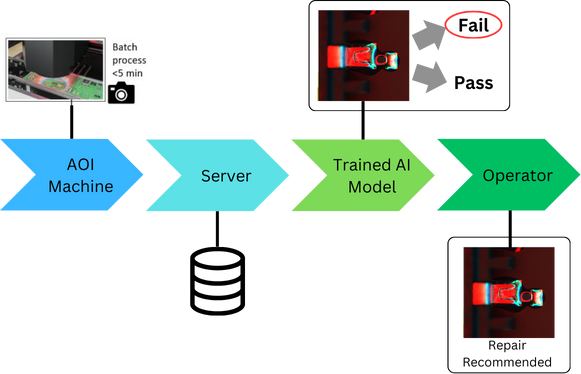
\includegraphics[width=1\linewidth]{Images/Solution_Pipeline.png}
    \caption{Current Siemens solution pipeline}
    \label{fig:solution pipeline}
\end{figure}

The current solution also involves human inspectors who verify the model's recommendations and make final repair decisions. The operator is responsible for verifying the model's prediction and making the final decision on whether a repair is needed or not. This manual intervention, while still necessary to ensure product quality, adds a layer of complexity and delay to the inspection process. As production demands increase, the dependence on human inspectors can become a bottleneck, preventing the desired levels of efficiency and throughput. Moreover, the manual nature of this process makes it difficult to achieve consistent inspection quality, as human inspectors may vary in their judgment and expertise.

Given these challenges, there is a clear need for an alternative approach to overcome the limitations associated with supervised learning. The unsupervised models explored in this thesis offer a promising solution by eliminating the need for labeled data and providing a more flexible, scalable approach to defect detection. Integrating an unsupervised anomaly detection model into the existing pipeline instead of the baseline \gls{yolo} model could significantly reduce the time and cost associated with labeling. 

\section{Thesis Objective}

The objective of this thesis is to develop a trained, unsupervised anomaly detection model for identifying faulty soldered pins in \gls{pcb} assemblies. This approach aims to reduce the dependency on manual labeling processes while maintaining high accuracy, thereby improving the scalability of the visual inspection process in electronics manufacturing. Specifically, this research seeks to:

\begin{enumerate}
    \item Evaluate the feasibility of using unsupervised anomaly detection models to identify defects in solder joints without requiring labeled datasets.

    \item Benchmark various models from the Anomalib library, PatchCore, \gls{dfm}, \gls{dfkde}, EfficientAD, and FastFlow, to assess their performance in anomaly detection.

    \item Optimize the model's performance through hyperparameter tuning and evaluate the models based on accuracy, precision, recall, and F1-score metrics.
\end{enumerate}

%\section{Thesis Outline}
%This thesis comprises of three main chapters: Theoretical Background, Methodology, and Results \& Discussion.

